%%%%%%%%%%%%%%%%%%%%%%%%%%%%%%%%%%%%%%%%%%%%%%%%%%%%%%%%%%%%%%%%%%%%%%%%%%%%%%%%
%2345678901234567890123456789012345678901234567890123456789012345678901234567890
%        1         2         3         4         5         6         7         8

%\documentclass[letterpaper, 10 pt, conference]{ieeeconf}  % Comment this line out if you need a4paper

\documentclass[a4paper, 10pt, conference]{ieeeconf}      % Use this line for a4 paper

\IEEEoverridecommandlockouts                              % This command is only needed if 
                                                          % you want to use the \thanks command

\overrideIEEEmargins                                      % Needed to meet printer requirements.

%In case you encounter the following error:
%Error 1010 The PDF file may be corrupt (unable to open PDF file) OR
%Error 1000 An error occurred while parsing a contents stream. Unable to analyze the PDF file.
%This is a known problem with pdfLaTeX conversion filter. The file cannot be opened with acrobat reader
%Please use one of the alternatives below to circumvent this error by uncommenting one or the other
%\pdfobjcompresslevel=0
%\pdfminorversion=4

% See the \addtolength command later in the file to balance the column lengths
% on the last page of the document

% The following packages can be found on http:\\www.ctan.org
\usepackage{graphicx} % for pdf, bitmapped graphics files
%\usepackage{epsfig} % for postscript graphics files
\usepackage{mathptmx} % assumes new font selection scheme installed
%\usepackage{times} % assumes new font selection scheme installed
\usepackage{amsmath} % assumes amsmath package installed
\usepackage{amssymb}  % assumes amsmath package installed
\usepackage{tikz}
\usepackage{multirow} % merge columns in rows

\title{\LARGE \bf
Generation of Complex Road Networks Using a Simplified Logical Description for the Validation of Automated Vehicles*
}


\author{Daniel Becker$^{1}$, Fabian Ru{\ss}$^{1}$ and Lutz Eckstein$^{2}$% <-this % stops a space
\thanks{*This research is funded by the SET Level 4to5 research initiative, promoted by the	Federal Ministry for Economic Affairs and Energy (BMWi).}% <-this % stops a space
\thanks{$^{1}$Daniel Becker and Fabian Ru{\ss} are with the automated driving department of the Institute for Automotive Engineering (ika), RWTH Aachen University, 52074 	Aachen, Germany {\tt\small \{daniel.becker, fabian.russ\}@ika.rwth-aachen.de}}%
\thanks{$^{2}$Lutz Eckstein is head of the Institute for Automotive Engineering (ika), RWTH Aachen University, 52074 Aachen, Germany {\tt\small lutz.eckstein@ika.rwth-aachen.de}}%
}

\begin{document}

\maketitle
\thispagestyle{empty}
\pagestyle{empty}

%%%%%%%%%%%%%%%%%%%%%%%%%%%%%%%%%%%%%%%%%%%%%%%%%%%%%%%%%%%%%%%%%%%%%%%%%%%%%%%%
\begin{abstract}
The verification and validation of automated driving functions is an essential building block in the process of releasing those functions to the public.  
\end{abstract}

%%%%%%%%%%%%%%%%%%%%%%%%%%%%%%%%%%%%%%%%%%%%%%%%%%%%%%%%%%%%%%%%%%%%%%%%%%%%%%%%
\section{INTRODUCTION}

To assure the safety of automated driving functions (ADF), verification and validation methods need to developed and established. (testfahrten und nötige km. etc erklären. zu Szenarien und simulation überleiten)

One approach to reach this state is scenario based testing. [ref] proposed different stages of scenarios: functional, logical and concrete. The term functional states a linguistic description which allows experts to talk about scenarios at an early stage of the development process. In logical scenarios parameters and ideally their probability distributions are provided. Finally, concrete scenarios specify a distinct value for each parameter which makes them feasible to be executed reproducible in a simulation or on proving grounds. Each stage can be divided into six levels (ref. EN layer ,hendrik) where the three lower layers describe the static part of the scenario, i.e. the road. Layer four focuses on moving objects, whereas layer five and six describe environmental conditions and vehicle-to-everything (V2X) communication, respectively. Detailed discussion in [ref hendrik eindhoven] (oder schreibt man das nicht?)

Current research initiatives such as SET Level 4to5 (footnote?) address simulative scenario based testing with focus on inner city traffic. Besides layer four which describes the dynamic behavior of all participants, the static scenery has to be taken into account as well. The latter is described within layer one to three and has to be defined in a logical and concrete manner, respectively. The open source standard format OpenDRIVE [ref asam] is suitable for concrete descriptions of road networks and is widely used in industry and research. However, by now there is no standardized logical road description format which is easy to use and capable to be transfered into OpenDRIVE. 

This article introduces a prototypical logical description language for complex road networks and a tool which generates concrete, standardized OpenDRIVE maps which may be used for the simulative testing of ADF. An example which outlines the idea of the concept is shown in Fig.~\ref{fig_motivation}

\begin{figure}[tpb] 		
	\centering
	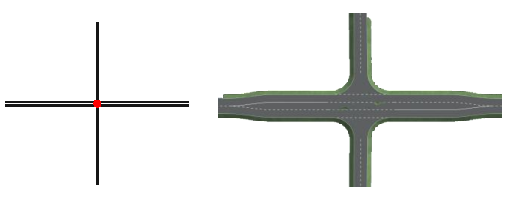
\includegraphics{fig/motivation.pdf}
	\caption{Graphical example of input and output of the road generation tool. As a minimal input two reference lines with assigned road types and a coupling point are sufficient to generate an intersection written in valid OpenDRIVE. (OpenDRIVE visualized in CarMaker 8.0[ref?]) \textbf{roughDraft}}
	\label{fig_motivation}
\end{figure}
%\begin{figure}
%	\begin{tikzpicture}
%	\node[anchor=west](layer6) at (0,7.4) {\small Layer 6};
%	\node[anchor=west](layer5) at (0,6.1) {\small Layer 5};
%	\node[anchor=west](layer4) at (0,4.9) {\small Layer 4};
%	\node[anchor=west](layer3) at (0,3.6) {\small Layer 3};
%	\node[anchor=west](layer2) at (0,2.3) {\small Layer 2};
%	\node[anchor=west](layer1) at (0,0.8) {\small Layer 1};
%	\begin{scope}[xshift=1.22cm]
%	\node[anchor=south west,inner sep=0] (image) at (0,0) {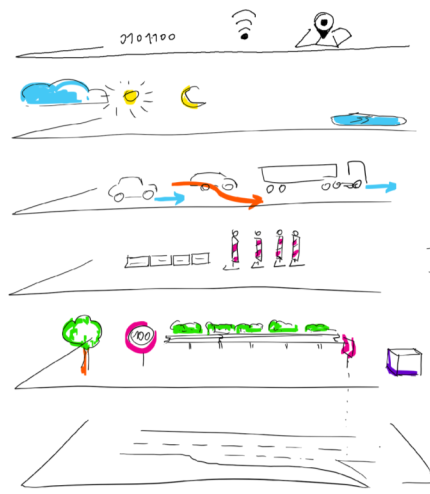
\includegraphics[width=0.4\textwidth]{fig/en_layers_raw.png}};
%	\end{scope}
%	\end{tikzpicture}
%	\caption{The data layers for the description of a scenario following~\cite{bock2018data} and~\cite{bagschik2018ontology}}
%	\label{fig:datalayers}
%\end{figure}
\section{RELATED WORK}
During the research initiative PEGASUS [ref] these concepts have been developed and utilized within the domain German motorway. Furthermore, the main focus has been on layer four. Nevertheless, when moving the testing domain to inner city scenarios such as the driving behavior on intersections, layers one to three are much more complex. Motorways usually consist of parallel lanes which follow curves with big radii. Such a road is not complicated to describe and generate. It can be done automatically with low effort. [ref. menzel et al.] propose a method to create a standardized road network in the OpenDRIVE format from a logical (and functional) road description. However, inner city intersections are more complex both in the logical description and in terms of the concrete format. 

die Frage ist, was alles "related" ist... eventuell kuerzer halten und laengere introduction? \textit{bibtex platzhalter} \cite{BagschikG..2018} \cite{Roesener2017}

\textit{hier muss noch der DLR ODR generator und deren logische Beschreibung für Autobahnen aus Pegasus rein \cite{dlrODRgen}}

\section{METHODOLOGY}
The concept presented in this paper aims to offer a description for road networks which allows easy modifications of the map due to a non-redundant design. Further, it is possible to provide limited information for intersections and lane definitions since some default configurations for main and access roads are defined. The input shall be translated into a concrete standardized road description format. With the logical description comes a road generation tool that calculates all required OpenDRIVE quantities from the simplified input. We use XML to store the input and the corresponding OpenDRIVE output is saved in XML as well. This way we attempt to close a gap in the pipeline of defining logical scenarios on intersections and make them executable in a concrete manner.

\section{LOGICAL ROAD DESCRIPTION}
The proposed logical road description is derived from the reference line concept used in OpenDRIVE [ref]. This means that each lane is described by an offset from a reference line defined in the x,y-plane (topview). However, in contrast to OpenDRIVE we introduce some simplifications and eliminate redundancies along the reference line. Each road segment consists of the geometric primitives line, arc and spiral, which is motivated by the federal guidelines for road constructions [ref]. A simplified illustration of the road network's XML structure is shown in Fig.~\ref{fig_schema}. On the first level under the \textit{roadNetwork} tag all segments are defined and links which connect them can be stated. In addition, "loose ends" of segments can be automatically connected inside the \textit{closeRoadNetwork} tag. As illustrated, segments might be T-/X-junctions, roundabouts and connection roads. 
\begin{figure}[thpb] 		
	\centering
	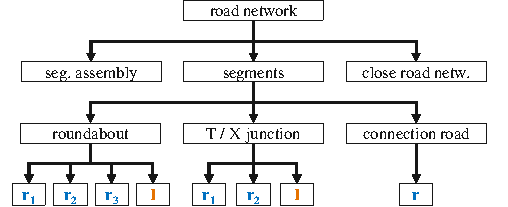
\includegraphics{fig/schema.pdf}
	\caption{Hierarchical structure of the road network. On the first level all segments and their relation to each other are defined. In addition, it is possible to define the automatic connection of two road ends. Segments are defined as roundabouts, junctions and connection roads. $r_i$ and $I$ describe roads and intersection definitions, respectively}
	\label{fig_schema}
\end{figure}
\subsection{Route Layout / Linienführung} % or find better heading
In order to ensure a smooth driveability along the road network, we define that the curvature has to be continuous along roads. Therefor, the definition of curvature over distance, a start point and initial heading is sufficient to uniquely describe a road segment's course (cf.~(\ref{eq1})). Fig.~\ref{fig_curvGraph} shows the definition of a road segment that is composed of the geometric primitive sequence line-spiral-arc-spiral-line.

As shown in Fig.~\ref{fig_curvGraph}, the curvature $\kappa(s)$ is a piecewise linear defined function over distance. Since we use lines, spirals and arcs, three definitions for those pieces are required. A line is described by $\kappa(s) = 0$, a spiral is characterized by a linear change of curvature: $\kappa(s) = a s$, where $a$ is constant (for details on spirals cf. [ref]). Finally, an arc's curvature is defined as: $\kappa(s) = \kappa_\text{arc}$, where $\kappa_\text{arc}$ is constant. Those definitions have their origin at $s=0$ and need to be shifted by their specific $s_\text{start}$ when being concatenated to a curvature graph. If the initial values $\phi_\text{0}, x_\text{0}, y_\text{0}$ are provided, the plan view coordinates can be calculated as follows:
\begin{equation} \label{eq1}
\begin{split}
\phi(s) &= \int_0^s \kappa(\hat{s}) d\hat{s} + \phi_\text{0} \\ 
x(s) &= \int_{0}^{s} \cos(\phi(\hat{s})) d\hat{s} + x_\text{0} \\ 
y(s) &= \int_{0}^{s} \sin(\phi(\hat{s})) d\hat{s} + y_\text{0} \\
\end{split}
\end{equation}
\begin{figure}%[thpb] 		
	\centering
	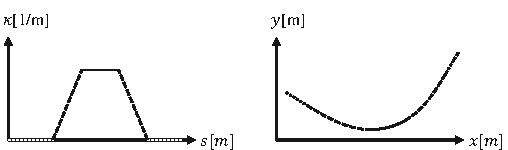
\includegraphics{fig/curvGraph.pdf}
	\caption{Example for a curve defined by the curvature graph. The plan view results from two integrations over $s$. Geometric primitives: line-spiral-arc-spiral-line. Positive curvature values correspond to left turns in positive $s$ direction.\textbf{roughDraft, wenn es zu viele Abb. werden, kann diese raus... Evtl. ersetzen durch eine Abb., die ref. Linie, Fahrstreifen und Objekte beinhaltet. Vgl. ODR}}
	\label{fig_curvGraph}
\end{figure}
\textit{briefly explain s,t coordinate system....}

\subsection{Connection Roads}
Connection roads consist of single \textit{road} tags defined by a reference line and definition for lanes and signals in the s,t-coordinate system. Lane extension and merging follow 3rd degree polynomials which are stated by their start and end point in s,t-coordinates, the corresponding polynomial coefficients are calculated by the road generation tool (\textit{Falls platz ist, kann noch eine Grafik mit Spuraufweitung erzeugt werden}).

\subsection{Junctions}
At least two and at most three \textit{road} entities are required to create a T-junction. Often one road is the dominant or main road in an intersection, which can be exploited by defining it as a single road that is intersected by an access road (cf. Fig.~\ref{fig_juncDef}). Alternatively, three single roads can be combined to form a T-junction by defining one reference road and the angles at which the other two roads are connected. In addition to topological information of the junction, it is possible to define the intersection area more detailed. First, for each road arm the distance from the intersection point to the beginning of the junction can be specified. The latter means the point where turning lanes start to leave the course of the reference line. Fig.~\ref{fig_createJunction} c) shows such an intersection area. Furthermore, additional lanes for left and right turns can be added ad libitum (\textit{verrückter ausdruck für "nach Belieben"}). Those lanes are specified by their minimal radius, the concrete course is calculated automatically. The descriptions of T- and X-junctions are a lot alike and thus X-junctions can be created analogously to the preceding paragraph about T-junctions.
\begin{figure}[thpb] 		
	\centering
	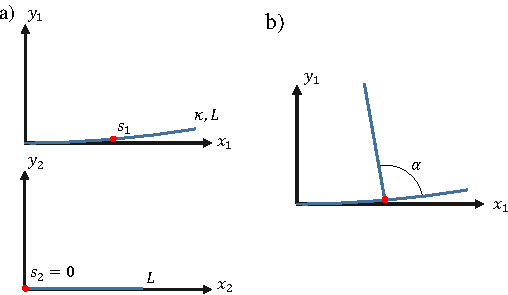
\includegraphics{fig/junctionDef.pdf}
	\caption{Two roads are coupled to form a T-junction. Road 1 is defined as an arc by length and curvature whereas road 2 is a straight line with length $L_l$. On both roads the intersection point along $s$ is defined. In addition, the angle $\alpha$ at this point is stated. }
	\label{fig_juncDef}
\end{figure}

\subsection{Road Network creation}
\textit{paragraph for concatenating road segments to a network}
\begin{figure}[thpb] 		
	\centering
	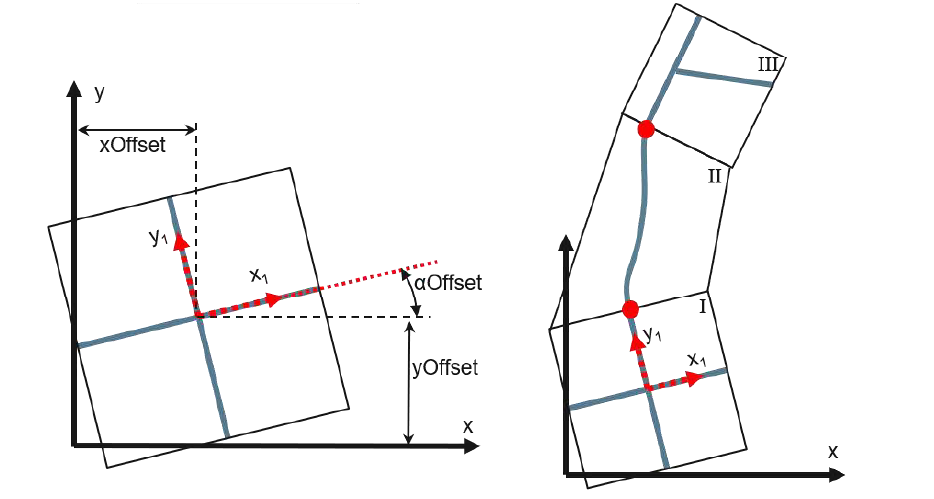
\includegraphics[width=0.9\columnwidth]{fig/concatSegments.png}
	\caption{Three segments are concatenated to form a road network. First, one reference segment has to be set (I). For further connections only the two end points need to be specified because concatenation follows the continuous curvature condition. \textbf{NEU MACHEN, Bsp gut so, aber Achsen und Schrift anpassen}}
	\label{fig_concatSeg}
\end{figure}

\subsection{Closing the raod network}

\section{ROAD GENERATION / IMPLEMENTATION}
\begin{figure}[thpb] 		
	\centering
	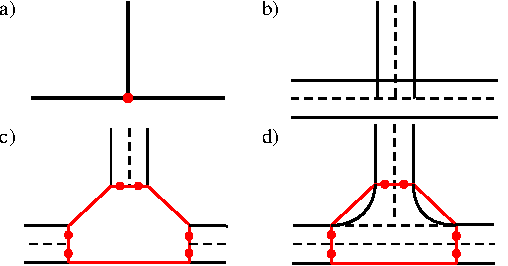
\includegraphics{fig/createJunction.pdf}
	\caption{From logical definition to concrete intersection. After the reference lines are in the correct position a), corresponding lanes are generated (b). Subsequently, the intersection area is cut free (c) and all required connection lanes are generated automatically (d). \textbf{grafik ok so...?}}
	\label{fig_createJunction}
\end{figure}

\section{RESULTS}

\begin{table}[h]
\caption{Comparison of OpenDRIVE and logical description}
\label{tab_comparison}
\def\arraystretch{1.5}
\begin{center}
\begin{tabular}{c|cccc}
\multirow{2}{*}{File} & \multicolumn{2}{c}{OpenDRIVE} & \multicolumn{2}{c}{Logical Description}\\
& Lines & Chars & Lines & Chars \\
\hline
1 & $23423$ & $23423$& $7\%$ &$9\%$\\
2 & $2343$ & $3423$& $7\%$ &$9\%$\\
3 & $3423$ & $1423$& $7\%$ &$9\%$
\end{tabular}
\end{center}
\end{table}

\section{CONCLUSIONS}

\addtolength{\textheight}{-12cm}   % This command serves to balance the column lengths
                                  % on the last page of the document manually. It shortens
                                  % the textheight of the last page by a suitable amount.
                                  % This command does not take effect until the next page
                                  % so it should come on the page before the last. Make
                                  % sure that you do not shorten the textheight too much.

%%%%%%%%%%%%%%%%%%%%%%%%%%%%%%%%%%%%%%%%%%%%%%%%%%%%%%%%%%%%%%%%%%%%%%%%%%%%%%%%



%%%%%%%%%%%%%%%%%%%%%%%%%%%%%%%%%%%%%%%%%%%%%%%%%%%%%%%%%%%%%%%%%%%%%%%%%%%%%%%%



%%%%%%%%%%%%%%%%%%%%%%%%%%%%%%%%%%%%%%%%%%%%%%%%%%%%%%%%%%%%%%%%%%%%%%%%%%%%%%%%

\bibliographystyle{IEEEtran}
\bibliography{IEEEexample,ma_russ,anonymization,roadgen}

\end{document}
